% ============================================================
%  Al-Haseeb Medical Health Care Center SKG — Business Plan
%  Course: Entrepreneurship & Business Management | BS CS | Sem 8
%
%  Compliance checklist (compile twice for TOC/refs):
%    • Body & quotations: 12 pt Times-like (mathptmx); black text only
%    • Outline numbered hierarchy: §1, §1.1, §1.1.1 (secnumdepth 3)
%    • Title page: hierarchy TitleCase / emphasis as coded below
%    • hyperref: links, cites, URLs render black (print-safe)
%    • Pagination: no printed page numbers through Executive Summary; Arabic from §1 (Introduction)
%    • Technical narrative aligned with repository (React+Vite, Express,
%      MongoDB, JWT, routes under frontend/src and backend/)
% ============================================================

\documentclass[12pt, a4paper]{article}

% --- Packages ---
\usepackage[top=1in, bottom=1in, left=1.2in, right=1.2in]{geometry}
\usepackage{mathptmx}
\usepackage[T1]{fontenc}
\usepackage{setspace}
\usepackage{titlesec}
\usepackage{booktabs}
\usepackage{array}
\usepackage{longtable}
\usepackage{graphicx}
\usepackage{tikz}
\usetikzlibrary{positioning}
\usepackage{fancyhdr}
\usepackage{enumitem}
\usepackage{parskip}
\usepackage{microtype}
\usepackage{url}
\usepackage{hyperref}

\hypersetup{
    colorlinks=true,
    linkcolor=black,
    urlcolor=black,
    citecolor=black,
    pdfborder={0 0 0}
}

% --- Outline numbering (numbered outline per academic report rules) ---
\setcounter{secnumdepth}{3}
\setcounter{tocdepth}{3}

% --- Heading styles: bold Title Case lines; rule under major sections only ---
%    Section = \large bold + number; Subsection = \normalsize bold + number;
%    Subsubsection = \normalsize italic + number (body remains 12 pt).
\titleformat{\section}{\large\bfseries}{\thesection}{0.75em}{}[\titlerule]
\titleformat{\subsection}{\normalsize\bfseries}{\thesubsection}{0.75em}{}
\titleformat{\subsubsection}{\normalsize\itshape}{\thesubsubsection}{0.75em}{}

\titlespacing{\section}{0pt}{18pt}{8pt}
\titlespacing{\subsection}{0pt}{12pt}{4pt}
\titlespacing{\subsubsection}{0pt}{8pt}{2pt}

% --- Header / Footer ---
\pagestyle{fancy}
\fancyhf{}
\fancyhead[L]{\small Al-Haseeb Medical Health Care Center SKG}
\fancyhead[R]{\small Business Plan --- March 2026}
\fancyfoot[C]{\small\thepage}
\renewcommand{\headrulewidth}{0.3pt}
\fancypagestyle{plain}{
  \fancyhf{}
  \fancyfoot[C]{\small\thepage}
  \renewcommand{\headrulewidth}{0pt}
}

% --- Table helper ---
\newcolumntype{L}[1]{>{\raggedright\arraybackslash}p{#1}}
\newcolumntype{C}[1]{>{\centering\arraybackslash}p{#1}}
\newcolumntype{R}[1]{>{\raggedleft\arraybackslash}p{#1}}

\setlength{\parindent}{0pt}
\setlength{\parskip}{6pt}
\onehalfspacing

% ============================================================
\begin{document}
\pagestyle{empty}

% ============================================================
%  TITLE PAGE
% ============================================================
\thispagestyle{empty}
\begin{center}

\vspace*{0.8cm}

% University logo: place \texttt{university_logo.png} or \texttt{university_logo.pdf} in the same folder as this .tex file (project root).
\IfFileExists{university_logo.png}{%
  \includegraphics[width=3.8cm]{university_logo.png}%
}{%
  \IfFileExists{university_logo.pdf}{%
    \includegraphics[width=3.8cm]{university_logo.pdf}%
  }{%
    \fbox{\parbox[c][2.8cm][c]{4.2cm}{\centering\small\textit{[University logo --- add \texttt{university\_logo.png} here]}}}%
  }%
}\\[1cm]

% Title page hierarchy: institution (uppercase) → tagline (italic) → document type → subtitle
{\LARGE\bfseries AL-HASEEB MEDICAL HEALTH CARE CENTER SKG}\\[6pt]
{\large\itshape ``Bringing Healthcare to Your Doorstep --- 24 Hours a Day''}

\vspace{1.2cm}
{\Large\bfseries BUSINESS PLAN}\\[4pt]
{\normalsize Full-Stack Web Application (React + Node.js API + MongoDB) --- Digital Outreach Initiative}

\vspace{1.5cm}
\noindent\rule{10cm}{0.4pt}

\vspace{1cm}
\begin{tabular}{ll}
\textbf{Submitted To:}   & Department of Computer Science \\[4pt]
\textbf{Submitted By:}   & Hassam Akram \quad|\quad Usman Awan \\[4pt]
\textbf{Course:}         & Entrepreneurship \& Business Management \\[4pt]
\textbf{Program:}        & BS Computer Science \\[4pt]
\textbf{Semester:}       & 8\textsuperscript{th} \\[4pt]
\textbf{Date:}           & March 2026 \\[4pt]
\textbf{Location:}       & Shakargarh (SKG), District Narowal, Punjab, Pakistan \\
\end{tabular}

\vspace{1.5cm}
\noindent\rule{10cm}{0.4pt}

\vfill
{\small Prepared as part of a student academic project — E\&BM / IT / System Analysis \& Design}

\end{center}

\newpage

% ============================================================
%  TABLE OF CONTENTS (no page number on this page or Title Page)
% ============================================================
\tableofcontents
\thispagestyle{empty}
\newpage

% ============================================================
%  ACKNOWLEDGEMENT
% ============================================================
\section*{Acknowledgement}
\addcontentsline{toc}{section}{Acknowledgement}

We express our sincere gratitude to our course instructor for the guidance provided throughout this project. We also thank the management and staff of Al-Haseeb Medical Health Care Center SKG for sharing operational details that made this business plan realistic and grounded. This project would not have been possible without the continued support of our families and colleagues.

Finally, we acknowledge the broader community of Shakargarh (SKG) and nearby areas whose healthcare needs inspired this initiative — and whose trust in local home healthcare services drives the purpose behind every page of this plan.

\newpage

% ============================================================
%  EXECUTIVE SUMMARY (unnumbered front matter; listed in TOC)
% ============================================================
\section*{Executive Summary}
\addcontentsline{toc}{section}{Executive Summary}

Al-Haseeb Medical Health Care Center SKG is a legally registered home healthcare business operating 24 hours a day, seven days a week, in Shakargarh (SKG), District Narowal, Punjab, Pakistan. It delivers a comprehensive range of medical services --- including injections, wound dressings, IV drips, blood sampling, and catheter care --- directly to patients in their homes.

Historically, outreach relied heavily on offline channels (flyers, referrals). This document aligns with the \textbf{implemented student repository}: a bilingual, mobile-first \textbf{React~(Vite)} front end with \textbf{Express} REST APIs, \textbf{MongoDB} persistence, \textbf{JWT}-secured admin tools, public booking and inquiry flows, and WhatsApp integration as coded under \texttt{frontend/src} and \texttt{backend/}.

The total one-time investment for design, integration, and deployment remains estimated at \textbf{PKR 30,000 -- 50,000}, recoverable within 2 to 5 months from incremental patient inquiries attributable to the digital channel.

Across all dimensions — market demand, technical feasibility, financial return, and operational manageability — the project is confirmed feasible and \textbf{approved for implementation}.

\newpage
\pagestyle{fancy}
\pagenumbering{roman}
\setcounter{page}{1}

% ============================================================
%  MISSION, VISION, LOGO \& TAGLINE (Roman numerals continue here)
% ============================================================
\section*{Mission, Vision, Logo \& Tagline}
\addcontentsline{toc}{section}{Mission, Vision, Logo \& Tagline}

\subsection*{Mission Statement}
To provide accessible, affordable, and professional home healthcare services to the residents of Shakargarh (SKG) and surrounding areas --- 24 hours a day, 7 days a week --- by bringing qualified medical care directly to patients in the comfort of their homes.

\subsection*{Vision Statement}
To become the most trusted and recognised home healthcare provider in the Narowal district, expanding digital reach so that every family in the region can access quality medical care with a single tap or call.

\subsection*{Logo \& Tagline}

\begin{center}
\textit{[Business Logo — To be inserted here]}\\[8pt]
\textbf{Tagline:} \textit{``Bringing Healthcare to Your Doorstep — 24 Hours a Day''}
\end{center}

\noindent The logo features a medical cross symbol paired with a home icon, reflecting the core identity of the clinic as a home-based healthcare service. The colour palette uses navy blue and white — conveying trust, cleanliness, and professionalism.

\newpage

% ============================================================
%  INTRODUCTION (Arabic page numbering starts here at page 1)
% ============================================================
\clearpage
\pagestyle{fancy}
\pagenumbering{arabic}
\setcounter{page}{1}

\section{Introduction}

\subsection{Introduction of Business}

Al-Haseeb Medical Health Care Center SKG is a home healthcare business providing round-the-clock medical services to patients in Shakargarh (SKG), District Narowal, Punjab, Pakistan. The clinic was established to address a clear gap in the local healthcare landscape: the difficulty faced by elderly, post-operative, and chronically ill patients in travelling to hospitals for routine medical care.

\subsection{Background of Business}

The clinic operates as a sole proprietorship, owned and managed by a single individual who oversees all operations, bears all financial responsibilities, and makes all key decisions. Before this full-stack web initiative, visibility relied mainly on word-of-mouth and printed flyers; the React/Express/MongoDB system described in this plan formalises digital reach and scales patient acquisition.

\subsection{Description of Business}

The clinic provides the following services, all delivered to patients at their homes:

\begin{itemize}[leftmargin=1.4em]
    \item Injections (intramuscular, subcutaneous, intravenous)
    \item Wound dressing and post-surgical care
    \item IV drip administration
    \item Blood pressure and blood sugar monitoring
    \item Foley catheter and NG tube care
    \item Blood sampling and basic laboratory tests
    \item 24-hour emergency home care
\end{itemize}

\subsection{Point of Uniqueness}

Al-Haseeb stands out from competitors through three core differentiators:

\begin{itemize}[leftmargin=1.4em]
    \item \textbf{24/7 availability} — unlike most local clinics, the center never closes
    \item \textbf{Home delivery of care} — patients avoid the burden of hospital travel
    \item \textbf{First-mover digital advantage} — no competing clinic in the area has an online presence, making this website a unique and powerful tool for patient acquisition
\end{itemize}

\newpage

% ============================================================
%  OPPORTUNITY ANALYSIS
% ============================================================
\section{Opportunity Analysis}

The Shakargarh (SKG) area and wider Narowal district have a significant population of elderly residents, post-operative patients, and individuals managing chronic illnesses. Travelling to hospitals for routine services is both physically challenging and financially burdensome for many families.

Key opportunity indicators include:

\begin{itemize}[leftmargin=1.4em]
    \item Rapid smartphone penetration in Punjab's semi-urban and rural areas, with most households owning at least one smartphone
    \item WhatsApp as the dominant communication channel in the local community — a website link shared via WhatsApp can reach hundreds of families instantly
    \item Growing volume of Google searches for terms such as \textit{``home nurse Shakargarh''}, \textit{``injection at home''}, and \textit{``blood test home service''}
    \item Zero competing clinics in the area with a digital presence — creating a first-mover advantage for Al-Haseeb
    \item Pakistan's increasing adoption of telehealth and digital health services at the national level, validating local demand
\end{itemize}

This combination of unmet local demand, growing digital usage, and an absence of online competitors represents a clear and time-sensitive business opportunity.

\newpage

% ============================================================
%  GOALS & OBJECTIVES
% ============================================================
\section{Goals \& Objectives}

\subsection{Short-Term Goals (Within 3 Months of Launch)}

\begin{itemize}[leftmargin=1.4em]
    \item Launch the website within 8 weeks of project kickoff
    \item Receive a minimum of 10 appointment form inquiries per month
    \item Register the clinic on Google Business Profile for local discoverability
    \item Share the website via WhatsApp to reach at least 500 local contacts in the first month
\end{itemize}

\subsection{Long-Term Goals (6–18 Months)}

\begin{itemize}[leftmargin=1.4em]
    \item Recover the full development cost (PKR 30,000–50,000) within 5 months
    \item Grow monthly patient inquiries to 30+ through organic SEO and referrals
    \item Expand the service menu listed on the website as new services are introduced
    \item Build a reputation as the leading digital home healthcare provider in the Narowal district
\end{itemize}

\subsection{Strategic Objectives}

\begin{itemize}[leftmargin=1.4em]
    \item \textbf{Customer Satisfaction:} Reduce patient waiting time through online appointment scheduling; collect feedback via WhatsApp to continuously improve service delivery
    \item \textbf{Innovation:} Introduce bilingual digital content (Urdu and English) — a first for any clinic in the local area
    \item \textbf{Value-Added Services:} Provide one-tap phone and WhatsApp access to medical staff, reducing friction in patient-clinic communication
\end{itemize}

\newpage

% ============================================================
%  PLANS TO ACHIEVE GOALS
% ============================================================
\section{Plans to Achieve Goals}

\subsection{Digital Strategy}
The React web application is the primary driver of patient acquisition. It is optimised for mobile devices (Android smartphones used locally). After deployment, the production URL will be submitted for indexing and registered on Google Business Profile with Shakargarh/Narowal locality data for map visibility.

\subsection{Community Outreach}
Staff members will share the website link via WhatsApp broadcast lists covering existing patients, community groups, and local networks. Physical QR codes linking to the website will be printed on updated flyers.

\subsection{Content \& SEO}
Service descriptions appear in both Urdu and English on the site (including Noto Nastaliq Urdu web fonts). Keywords such as ``home nurse Shakargarh'', ``24-hour home care SKG'', and ``injection at home Punjab'' are reflected in page titles, meta descriptions, and headings in \texttt{index.html} and routed pages.

\subsection{Monitoring \& Improvement}
The admin dashboard (MongoDB-backed) provides appointment and inquiry counts and recent activity for clinic oversight. Optional third-party analytics (e.g.\ Google Analytics) may be added to the React build later for traffic sources. Appointment requests submitted via \texttt{/booking} will be reviewed daily through the admin panel. Any technical issues reported by patients will be corrected within 48 hours.

\newpage

% ============================================================
%  INDUSTRY ANALYSIS
% ============================================================
\section{Industry Analysis}

\subsection{Overview of the Industry}

Home healthcare is a growing segment of Pakistan's broader healthcare industry. It addresses the critical gap between hospital-based care and patient needs at home — particularly for elderly, post-surgical, and chronically ill individuals. In Punjab, rising urban congestion, transport costs, and hospital queues have accelerated demand for home-based medical services.

\subsection{Competitors}

Al-Haseeb operates in a local market with limited direct competition. Competing providers in the Shakargarh (SKG) area include:

\begin{itemize}[leftmargin=1.4em]
    \item Small informal nursing services operating through personal referrals with no fixed service menu or pricing
    \item Hospital outreach teams offering limited home visits during business hours only
    \item None of the known competitors maintain a website or any form of digital presence
\end{itemize}

This creates a structural advantage for Al-Haseeb upon launching its website.

\subsection{Market Trends}

\begin{itemize}[leftmargin=1.4em]
    \item Pakistan's digital health sector is expanding, supported by government telemedicine initiatives
    \item Rural and semi-urban Punjab is experiencing rapid mobile internet adoption
    \item Consumer preference is shifting toward convenience-based healthcare services
    \item WhatsApp-based business communication is now standard across all economic segments in the region
\end{itemize}

\newpage

% ============================================================
%  MACRO ENVIRONMENT ANALYSIS (PEST)
% ============================================================
\section{Macro Environment Analysis (PEST)}

\begin{longtable}{@{} L{3.2cm} L{11.2cm} @{}}
\toprule
\textbf{Factor} & \textbf{Analysis} \\
\midrule
\endfirsthead
\toprule
\textbf{Factor} & \textbf{Analysis} \\
\midrule
\endhead
\textbf{Political} &
Pakistan's healthcare sector is governed by the Punjab Health Department. Home healthcare services operated by registered practitioners are legally permitted. The government's push towards digital Pakistan and e-governance creates a supportive regulatory environment for online business presence. \\[6pt]
\textbf{Economic} &
Pakistan faces economic challenges including inflation and rising hospital costs, which actually increase demand for affordable home-based care. The clinic's services are priced lower than equivalent hospital visits, positioning it well in the current economic climate. The website's low development cost (PKR 30,000–50,000) is appropriate for a sole proprietorship. \\[6pt]
\textbf{Social} &
The local population strongly prefers home-based care for elderly and post-operative patients due to cultural values around family caregiving. There is growing awareness of professional home nursing services. WhatsApp is deeply embedded in local communication, making digital outreach via this channel highly effective. \\[6pt]
\textbf{Technological} &
Smartphone penetration in Punjab is accelerating. 3G and 4G connectivity reaches semi-urban areas including Shakargarh (SKG). Google Search is increasingly used to find local services. The implemented solution uses a \textbf{React~19 single-page application} (Vite build tool, React Router), \textbf{Bootstrap~5} layout via CDN, custom CSS, and a \textbf{Node.js Express REST API} with \textbf{MongoDB} (Mongoose) and \textbf{JWT}-based authentication---technologies aligned with the BS~CS project stack and deployable on affordable shared hosting or a small VPS. \\
\bottomrule
\caption{PEST Analysis — Al-Haseeb Medical Health Care Center SKG}
\end{longtable}

\newpage

% ============================================================
%  ORGANIZATIONAL PLAN
% ============================================================
\section{Organizational Plan}

\subsection{Form of Business}

Al-Haseeb Medical Health Care Center SKG operates as a \textbf{sole proprietorship}. It is owned and managed by a single individual who invests capital, manages operations, and bears all business responsibilities. This structure is ideal for its scale — it requires no complex legal formalities, allows rapid decision-making, and keeps operational costs low.

\subsection{Roles \& Responsibilities}

\begin{longtable}{@{} L{3.5cm} L{10.9cm} @{}}
\toprule
\textbf{Role} & \textbf{Responsibilities} \\
\midrule
\endfirsthead
\toprule
\textbf{Role} & \textbf{Responsibilities} \\
\midrule
\endhead
Clinic Owner (Top Manager) &
Approves the website project; signs off on design and content; manages the annual hosting and domain budget; sets the overall strategic direction of the business. \\[6pt]
Web Developer (Middle Manager) &
Bridges the owner's vision and technical execution; coordinates React and Node milestones; implements fixes and features informed by admin dashboard usage and staff feedback. \\[6pt]
Healthcare Staff (5 Members) &
Respond to appointment form inquiries daily; share the website via WhatsApp; deliver home healthcare services; report technical issues raised by patients. \\
\bottomrule
\caption{Roles and Responsibilities}
\end{longtable}

\subsection{Decision-Making Process}

All major decisions — including website approval, pricing changes, and service additions — are made by the clinic owner. Day-to-day operational decisions (responding to inquiries, scheduling appointments) are delegated to healthcare staff.

\subsection{Termination Policy}

As a sole proprietorship, the business may be wound up at the discretion of the owner. In the event of closure, the website domain and hosting will be cancelled, patient records will be securely archived, and outstanding service obligations will be fulfilled before cessation.

\subsection{Organizational Structure}

\begin{center}
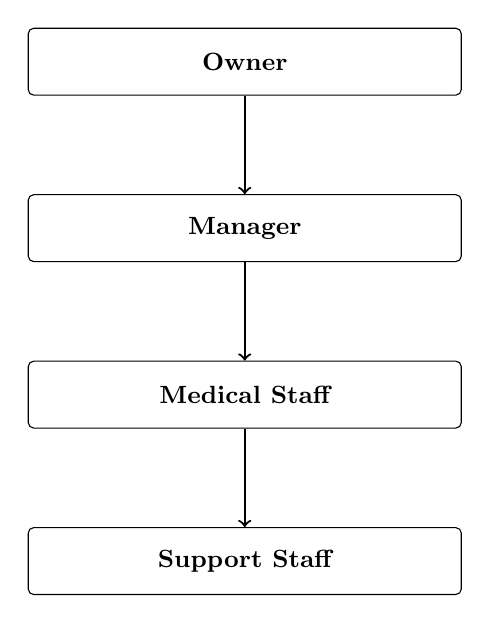
\begin{tikzpicture}[
  node distance=1.25cm,
  box/.style={rectangle, draw, rounded corners=2pt, minimum width=5.5cm, minimum height=0.85cm, align=center, font=\small\bfseries},
]
\node[box] (owner) {Owner};
\node[box, below=of owner] (manager) {Manager};
\node[box, below=of manager] (medical) {Medical Staff};
\node[box, below=of medical] (support) {Support Staff};
\draw[->, thick] (owner) -- (manager);
\draw[->, thick] (manager) -- (medical);
\draw[->, thick] (medical) -- (support);
\end{tikzpicture}\\[10pt]
{\small Clinic Owner $\rightarrow$ Web Developer $\rightarrow$ Healthcare Staff (×5)}
\end{center}

\subsection{Four Functions of Management}

\begin{longtable}{@{} L{3cm} L{11.4cm} @{}}
\toprule
\textbf{Function} & \textbf{Application} \\
\midrule
\endfirsthead
\toprule
\textbf{Function} & \textbf{Application} \\
\midrule
\endhead
Planning &
Defining the goal of launching the website; identifying target patients; setting an 8-week development timeline; establishing a budget of PKR 30,000–50,000. \\[6pt]
Organizing &
Assigning responsibilities to five healthcare staff for appointment responses; designating the web developer for technical build; allocating resources for domain, hosting, and content. \\[6pt]
Leading &
Motivating staff to adopt digital tools; training all team members in under two hours; encouraging the community to use the website for 24-hour healthcare access. \\[6pt]
Controlling &
Monitoring appointment and inquiry volumes via the admin dashboard; reviewing pending bookings daily; renewing hosting/domain and MongoDB subscription annually; fixing technical issues reported by patients. \\
\bottomrule
\caption{Four Functions of Management Applied to the Website Project}
\end{longtable}

\newpage

% ============================================================
%  OPERATIONAL / PRODUCTION PLAN
% ============================================================
\section{Operational Plan}

\subsection{Service Delivery Process}

Al-Haseeb's core operation involves receiving a patient request (via phone, WhatsApp, or website form), dispatching a qualified healthcare professional to the patient's home, delivering the required service, and following up as needed.

\subsection{Website Development Process (As Implemented in the Repository)}

The deliverable is a \textbf{client--server web application}, not a static HTML brochure. The \textbf{frontend} is a React~19 application scaffolded with \textbf{Vite}, using \textbf{React Router} for routes, \textbf{Axios} for HTTP calls to the backend, and \textbf{React Hook Form} for validated booking and contact forms. Styling combines \textbf{Bootstrap~5} (CDN) with project-specific CSS; icons use Bootstrap Icons. Urdu typography uses \textbf{Noto Nastaliq Urdu} from Google Fonts alongside the Latin \textbf{Outfit} family in \texttt{index.html}.

The \textbf{backend} is an \textbf{Express} server exposing JSON REST endpoints under \texttt{/api}, connected to \textbf{MongoDB} via \textbf{Mongoose}. Passwords are hashed with \textbf{bcrypt}; admin and patient sessions use \textbf{JSON Web Tokens (JWT)} with protected routes for dashboard and content management.

\textbf{Public routes (no login)} include the Home landing page (with embedded Google Maps for Shakargarh), dedicated pages for About, Services, Pricing, and Contact, and \textbf{Book Appointment} (\texttt{/booking}) where patients submit name, phone, service type (datalist populated from live services API), preferred date/time, address, optional notes, and an emergency flag.

\textbf{Patient-facing auth:} Register and Login (\texttt{/signup}, \texttt{/login}) call \texttt{/api/auth/register} and \texttt{/api/auth/login}; \texttt{/api/auth/me} returns the current user when authenticated.

\textbf{Admin console} (\texttt{/admin}, JWT-protected): Dashboard overview with statistics and recent activity; \textbf{Appointments} management (list/update/delete); \textbf{Services} manager (CRUD so pricing pages stay in sync with the database); \textbf{Settings}. Admin login uses \texttt{/api/admin/login}.

\textbf{Lead capture:} Contact section posts to \texttt{/api/inquiries}; appointments post to \texttt{/api/appointments}. Both persist to MongoDB for staff review in the admin UI.

\textbf{UX affordances matching the live site:} floating WhatsApp button, mobile sticky call/WhatsApp bar, \texttt{tel:} and \texttt{wa.me} links (clinic number \texttt{03088053238}), and 24/7 messaging on the hero section.

\subsection{Resources Used}

\begin{itemize}[leftmargin=1.4em]
    \item \textbf{Human:} Full-stack developer (React + Node), clinic owner, five healthcare staff
    \item \textbf{Technical:} Domain (.com.pk / .pk); hosting suitable for static React build + Node API + MongoDB (e.g.\ VPS or PaaS); environment variables for \texttt{JWT} secrets and \texttt{MONGODB\_URI}; \texttt{VITE\_API\_URL} for production API base URL
    \item \textbf{Content:} Urdu and English strings in components; services maintained via admin Services Manager; Google Maps iframe on Home
    \item \textbf{Tools:} MongoDB Compass or host dashboard for data; admin dashboard for operational metrics; WhatsApp for outreach; optional Google Business Profile and future analytics tags
\end{itemize}

\subsection{Website Information Architecture (Site Structure)}

The production app uses \textbf{React Router} with a shared \texttt{MainLayout} (navbar, footer, floating WhatsApp, mobile sticky bar). \textbf{Public routes:} \texttt{/} Home (hero with 24/7 badge, links to \texttt{/booking}, WhatsApp deep link, sections for About, Pricing, Contact, testimonials, embedded Google Map for Shakargarh); \texttt{/about}; \texttt{/services}; \texttt{/pricing}; \texttt{/contact}; \texttt{/booking} (appointment form backed by API); \texttt{/login} and \texttt{/signup} for patient accounts. \textbf{Admin routes} under \texttt{/admin/login} and \texttt{/admin} (nested): Dashboard, Appointments, Services, Settings---protected by JWT. This matches the repository structure (\texttt{App.jsx}) and keeps navigation shallow for mobile users.

\subsection{Functional Features Aligned with the Project}

Table~\ref{tab:web-features} maps \textbf{implemented} frontend and backend capabilities in the repository to business outcomes (trust, leads, operations).

\begin{longtable}{@{} L{4.5cm} L{9.9cm} @{}}
\toprule
\textbf{Feature / Module} & \textbf{Description \& Repository Mapping} \\
\midrule
\endfirsthead
\toprule
\textbf{Feature / Module} & \textbf{Description \& Repository Mapping} \\
\midrule
\endhead
React SPA + Vite &
Single-page app with fast dev/build workflow; routes for marketing pages and tools listed in \texttt{App.jsx}. \\[6pt]
Bootstrap~5 + custom CSS &
Responsive grid and components; consistent with \texttt{index.html} CDN links and project stylesheets. \\[6pt]
Urdu + Latin typography &
\texttt{Noto Nastaliq Urdu} and \texttt{Outfit} fonts linked in \texttt{index.html}; supports bilingual content strategy. \\[6pt]
\texttt{tel:} \& WhatsApp (\texttt{wa.me}) &
Hero, navbar, footer, and floating widgets link to \texttt{03088053238} and WhatsApp chat templates. \\[6pt]
Appointment API &
\texttt{POST /api/appointments} stores bookings from \texttt{Booking.jsx}; fields include patient name, phone, service type (datalist from \texttt{GET /api/services}), date, time, address, notes, emergency flag. \\[6pt]
Contact inquiries API &
\texttt{POST /api/inquiries} from Contact section; persists leads for admin review. \\[6pt]
Dynamic services catalogue &
\texttt{GET /api/services} (public); admin \texttt{POST/PUT/DELETE /api/services/:id} keeps Services and booking datalist current. \\[6pt]
Patient authentication &
\texttt{/api/auth/register}, \texttt{/api/auth/login}, \texttt{/api/auth/me}; roles include Patient/Admin/SuperAdmin per user model. \\[6pt]
Admin dashboard &
\texttt{/api/dashboard/stats}, \texttt{/api/dashboard/recent-activity}; UI in \texttt{DashboardOverview.jsx}. \\[6pt]
Appointment \& inquiry management &
Protected list/update/delete for appointments; inquiry inbox for staff (\texttt{appointmentController}, \texttt{inquiryController}). \\[6pt]
JWT + bcrypt &
\texttt{protect} / \texttt{requireAdmin} middleware; hashed passwords; Axios interceptor attaches Bearer token for admin calls. \\[6pt]
Google Maps embed &
Iframe on Home pointing to Shakargarh area---matches footer contact copy (District Narowal). \\[6pt]
Pricing page &
Public \texttt{/pricing} aligned with Section~\ref{sec:pricing}; marketing copy references distance from Shakargarh base. \\[6pt]
Mobile UX widgets &
\texttt{WhatsAppFloat.jsx}, \texttt{MobileStickyBar.jsx} for persistent conversion paths on small screens. \\[6pt]
SEO meta tags &
\texttt{meta name="description"} and title in \texttt{index.html}; hash navigation on Home for section scrolling. \\[6pt]
Production configuration &
\texttt{VITE\_API\_URL} switches API base from localhost to deployed backend; CORS enabled on Express for the SPA origin. \\
\bottomrule
\caption{Website features aligned with the Al-Haseeb repository implementation}
\label{tab:web-features}
\end{longtable}

\subsection{Non-Functional Requirements}

\begin{itemize}[leftmargin=1.4em]
    \item \textbf{Compatibility:} Modern evergreen browsers; smoke-test React routes in WhatsApp in-app browser on Android.
    \item \textbf{Performance:} Optimised production build via \texttt{vite build}; image hygiene on hero assets; Axios 15\,s timeout per \texttt{api.js}.
    \item \textbf{Maintainability:} Component-based React codebase; services and appointments editable without code redeploy via admin APIs where applicable.
    \item \textbf{Security:} HTTPS in production; JWT secret in environment variables; never commit \texttt{.env} to version control.
    \item \textbf{Privacy \& data minimisation:} Store only inquiry and appointment fields required for scheduling; restrict admin routes to authenticated roles.
\end{itemize}

\subsection{Alignment with Offline Workflow}

Digital inquiries and API-created appointments appear in the \textbf{admin console} for the same triage workflow as phone and WhatsApp. Staff confirm timing and dispatch caregivers; the emergency checkbox on the booking form flags urgent requests. The application augments---not replaces---clinical judgement and formal emergency services when life-threatening conditions arise.

\newpage

% ============================================================
%  MARKETING PLAN
% ============================================================
\section{Marketing Plan}

\subsection{Target Patients (Product/Service Categories)}

\begin{longtable}{@{} L{5cm} L{9.4cm} @{}}
\toprule
\textbf{Patient Segment} & \textbf{Service Required} \\
\midrule
\endfirsthead
\toprule
\textbf{Patient Segment} & \textbf{Service Required} \\
\midrule
\endhead
Elderly patients & Routine injections, blood pressure checks \\[4pt]
Post-surgery patients & Wound dressing, IV drips at home \\[4pt]
Bedridden patients & Foley catheter and NG tube care \\[4pt]
Emergency families & Fast 24-hour home care dispatch \\[4pt]
Hospital-averse patients & Lab tests and blood sampling at home \\
\bottomrule
\caption{Target Patient Segments and Services}
\end{longtable}

\noindent\textbf{Image placeholders (product/service categories)}\\[6pt]
\fbox{\parbox[c][2.6cm][c]{0.97\textwidth}{\centering\small\textit{[Insert image: Elderly patients --- routine injections / vitals]}}}\\[8pt]
\fbox{\parbox[c][2.6cm][c]{0.97\textwidth}{\centering\small\textit{[Insert image: Post-surgery patients --- wound care / IV at home]}}}\\[8pt]
\fbox{\parbox[c][2.6cm][c]{0.97\textwidth}{\centering\small\textit{[Insert image: Bedridden patients --- catheter / NG care]}}}\\[8pt]
\fbox{\parbox[c][2.6cm][c]{0.97\textwidth}{\centering\small\textit{[Insert image: Emergency families --- 24-hour dispatch]}}}\\[8pt]
\fbox{\parbox[c][2.6cm][c]{0.97\textwidth}{\centering\small\textit{[Insert image: Hospital-averse patients --- lab / blood sampling at home]}}}

\subsection{Place — Distribution Channels}

Services are delivered directly to patients' homes across Shakargarh (SKG) and nearby areas. Patient acquisition channels are:

\begin{itemize}[leftmargin=1.4em]
    \item \textbf{Digital:} Website (primary new channel), Google Search, Google Business Profile
    \item \textbf{Social:} WhatsApp broadcast lists shared by staff and existing patients
    \item \textbf{Physical:} Updated printed flyers with website URL and QR code
\end{itemize}

\subsection{Promotion}

Promotional materials to be produced alongside the website launch:

\begin{itemize}[leftmargin=1.4em]
    \item \textbf{Brochures:} Bilingual (Urdu/English) A5 brochures listing all services and contact details
    \item \textbf{Flex banners:} Printed at key local intersections with clinic name, tagline, and WhatsApp number
    \item \textbf{Flyers:} A6 flyers with QR code linking to the website for distribution in local markets
    \item \textbf{WhatsApp broadcast:} Website link shared to all existing patient contacts on launch day
\end{itemize}

\subsection{Pricing Strategy}

Pricing follows a \textbf{competitive penetration strategy} — services are priced lower than hospital equivalents to attract cost-sensitive patients and build market share rapidly. Pricing is transparent and publicly visible on the website.

\subsection{Selling Techniques}

\begin{itemize}[leftmargin=1.4em]
    \item One-tap WhatsApp and phone buttons on the website eliminate friction at the point of patient decision
    \item 24-hour availability badge builds confidence in service reliability
    \item Bilingual content ensures accessibility for Urdu-speaking patients who may not be comfortable with English-only websites
\end{itemize}

\newpage

% ============================================================
%  PRICING TABLE
% ============================================================
\section{Pricing Table}\label{sec:pricing}

\begin{longtable}{@{} L{8cm} R{6.4cm} @{}}
\toprule
\textbf{Service} & \textbf{Price (PKR)} \\
\midrule
\endfirsthead
\toprule
\textbf{Service} & \textbf{Price (PKR)} \\
\midrule
\endhead
Injection (IM / SC / IV) & 300 – 500 \\[4pt]
Wound Dressing (simple) & 500 – 800 \\[4pt]
Wound Dressing (complex / post-surgical) & 800 – 1,500 \\[4pt]
IV Drip Administration & 700 – 1,200 \\[4pt]
Blood Pressure / Sugar Check & 200 – 300 \\[4pt]
Blood Sampling (at home) & 400 – 600 \\[4pt]
Foley Catheter Care & 800 – 1,200 \\[4pt]
NG Tube Care & 800 – 1,200 \\[4pt]
24-Hour Emergency Home Visit & 1,000 – 2,000 \\
\midrule
\textit{Average service value} & \textit{approx. PKR 1,500} \\
\bottomrule
\caption{Service Pricing — Al-Haseeb Medical Health Care Center SKG}
\end{longtable}

\textit{Note: Prices are estimates based on local market rates and may be adjusted by the clinic owner.}

\newpage

% ============================================================
%  FINANCIAL PLAN
% ============================================================
\section{Financial Plan}\label{sec:financial}

\subsection{Sources of Funds}

\begin{longtable}{@{} L{8cm} R{6.4cm} @{}}
\toprule
\textbf{Source} & \textbf{Capital Invested (PKR)} \\
\midrule
\endfirsthead
\toprule
\textbf{Source} & \textbf{Capital Invested (PKR)} \\
\midrule
\endhead
Clinic Owner (Personal Savings) & 30,000 – 50,000 \\
\midrule
\textbf{Total} & \textbf{30,000 – 50,000} \\
\bottomrule
\caption{Sources of Funds Table}
\end{longtable}

\subsection{Product Manufacturing Cost}

\begin{longtable}{@{} L{9cm} R{5.4cm} @{}}
\toprule
\textbf{Cost Item (service preparation / consumables)} & \textbf{Estimated Monthly (PKR)} \\
\midrule
\endfirsthead
\toprule
\textbf{Cost Item (service preparation / consumables)} & \textbf{Estimated Monthly (PKR)} \\
\midrule
\endhead
Dressings, syringes, basic consumables (bundled estimate) & 4,000 -- 8,000 \\[4pt]
IV setup consumables (share of monthly use) & 2,000 -- 5,000 \\
\midrule
\textbf{Total (indicative monthly manufacturing / preparation cost)} & \textbf{6,000 -- 13,000} \\
\bottomrule
\caption{Product Manufacturing Cost}
\end{longtable}

\subsection{Product Purchasing Cost}

\begin{longtable}{@{} L{9cm} R{5.4cm} @{}}
\toprule
\textbf{Purchasing Item} & \textbf{Estimated Cost (PKR)} \\
\midrule
\endfirsthead
\toprule
\textbf{Purchasing Item} & \textbf{Estimated Cost (PKR)} \\
\midrule
\endhead
Medical supplies inventory (initial stock-up) & 8,000 -- 15,000 \\[4pt]
Portable equipment maintenance / calibration (annual share) & 3,000 -- 6,000 \\
\midrule
\textbf{Total Product Purchasing Cost (indicative)} & \textbf{11,000 -- 21,000} \\
\bottomrule
\caption{Product Purchasing Cost}
\end{longtable}

\subsection{One-Time Website Development Costs}

\begin{longtable}{@{} L{9cm} R{5.4cm} @{}}
\toprule
\textbf{Item} & \textbf{Cost (PKR)} \\
\midrule
\endfirsthead
\toprule
\textbf{Item} & \textbf{Cost (PKR)} \\
\midrule
\endhead
Domain registration (.com.pk / .pk) & 2,000 – 3,000 \\[4pt]
Shared web hosting (1 year) & 5,000 – 8,000 \\[4pt]
Website design and development & 15,000 – 25,000 \\[4pt]
Urdu content writing and translation & 2,000 – 4,000 \\[4pt]
Photography of team and clinic & 3,000 – 5,000 \\[4pt]
SEO setup and Google Business registration & 2,000 – 3,000 \\[4pt]
Testing and quality assurance & 1,000 – 2,000 \\
\midrule
\textbf{Total One-Time Cost} & \textbf{30,000 – 50,000} \\
\bottomrule
\caption{One-Time Website Development Costs}
\end{longtable}

\subsection{Annual Recurring Costs}

\begin{longtable}{@{} L{9cm} R{5.4cm} @{}}
\toprule
\textbf{Item} & \textbf{Cost per Year (PKR)} \\
\midrule
\endfirsthead
\toprule
\textbf{Item} & \textbf{Cost per Year (PKR)} \\
\midrule
\endhead
Domain renewal & 2,000 – 3,000 \\[4pt]
Hosting renewal & 5,000 – 8,000 \\[4pt]
Minor content updates & 2,000 – 4,000 \\
\midrule
\textbf{Total Annual Recurring Cost} & \textbf{9,000 – 15,000} \\
\bottomrule
\caption{Annual Recurring Costs}
\end{longtable}

\subsection{Marketing Costs}

\begin{longtable}{@{} L{9cm} R{5.4cm} @{}}
\toprule
\textbf{Item} & \textbf{Cost (PKR)} \\
\midrule
\endfirsthead
\toprule
\textbf{Item} & \textbf{Cost (PKR)} \\
\midrule
\endhead
Flex banners (printed) & 2,000 – 3,500 \\[4pt]
Brochures (A5, bilingual) & 1,500 – 2,500 \\[4pt]
Flyers with QR code & 1,000 – 1,500 \\[4pt]
Logo stickers & 500 – 1,000 \\[4pt]
Standee (entrance display) & 2,000 – 3,000 \\
\midrule
\textbf{Total Marketing Cost} & \textbf{7,000 – 11,500} \\
\bottomrule
\caption{Total Marketing Cost}
\end{longtable}

\subsection{Total Project Cost Summary}

\begin{longtable}{@{} L{9cm} R{5.4cm} @{}}
\toprule
\textbf{Category} & \textbf{Cost (PKR)} \\
\midrule
\endfirsthead
\toprule
\textbf{Category} & \textbf{Cost (PKR)} \\
\midrule
\endhead
Website development (one-time) & 30,000 – 50,000 \\[4pt]
Marketing materials & 7,000 – 11,500 \\[4pt]
Annual recurring (Year 1 included) & 9,000 – 15,000 \\
\midrule
\textbf{Total Estimated Project Cost} & \textbf{46,000 – 76,500} \\
\bottomrule
\caption{Total Project Cost Summary}
\end{longtable}

\subsection{Projected Sales}

\begin{longtable}{@{} L{5.5cm} C{2.5cm} C{3cm} R{3.4cm} @{}}
\toprule
\textbf{Scenario} & \textbf{Price (PKR)} & \textbf{New Visits/Month} & \textbf{Annual Revenue (PKR)} \\
\midrule
\endfirsthead
\toprule
\textbf{Scenario} & \textbf{Price (PKR)} & \textbf{New Visits/Month} & \textbf{Annual Revenue (PKR)} \\
\midrule
\endhead
Conservative & 1,500 & 2 & 36,000 \\[4pt]
Moderate & 1,500 & 5 & 90,000 \\[4pt]
Optimistic & 1,500 & 10 & 180,000 \\
\bottomrule
\caption{Projected Sales Table}
\end{longtable}

\noindent The one-time development cost is recovered within \textbf{2 to 5 months} under even the most conservative scenario.

\subsection{Estimated Income Statement}

\begin{longtable}{@{} L{10cm} R{4.4cm} @{}}
\toprule
\textbf{Item} & \textbf{Amount (PKR)} \\
\midrule
\endfirsthead
\toprule
\textbf{Item} & \textbf{Amount (PKR)} \\
\midrule
\endhead
Total Estimated Annual Sales (moderate scenario) & 90,000 \\[4pt]
Less: Total Annual Expenses (recurring + marketing) & 26,500 \\
\midrule
\textbf{Estimated Net Profit (Year 1)} & \textbf{63,500} \\
\bottomrule
\caption{Estimated Income Statement (Year 1 — Moderate Scenario)}
\end{longtable}

\textit{Note: Development cost (one-time) excluded from Year 1 income statement as it is a capital outlay.}

\subsection{Pro-Forma Balance Sheet}

\begin{longtable}{@{} L{5.2cm} R{2.8cm} L{5.2cm} R{2.8cm} @{}}
\toprule
\textbf{Assets} & \textbf{PKR} & \textbf{Liabilities \& Equity} & \textbf{PKR} \\
\midrule
\endfirsthead
\toprule
\textbf{Assets} & \textbf{PKR} & \textbf{Liabilities \& Equity} & \textbf{PKR} \\
\midrule
\endhead
Website (intangible asset) & 40,000 & External Liabilities & Nil \\[4pt]
Cash in hand / bank & 23,500 & Owner's Capital & 50,000 \\[4pt]
Marketing materials & 9,000 & Retained Earnings & 22,500 \\
\midrule
\textbf{Total Assets} & \textbf{72,500} & \textbf{Total Liabilities \& Equity} & \textbf{72,500} \\
\bottomrule
\caption{Pro-Forma Balance Sheet (End of Year 1 — Moderate Scenario)}
\end{longtable}

\subsection{Pro-Forma Cash Flow Statement}

\begin{longtable}{@{} L{9cm} R{5.4cm} @{}}
\toprule
\textbf{Item} & \textbf{PKR} \\
\midrule
\endfirsthead
\toprule
\textbf{Item} & \textbf{PKR} \\
\midrule
\endhead
\textbf{Operating Activities} & \\[2pt]
Cash inflow from patient services & 90,000 \\[4pt]
Less: Annual recurring expenses & (15,000) \\[4pt]
Less: Marketing costs & (11,500) \\
\midrule
Net Cash from Operating Activities & 63,500 \\[6pt]
\textbf{Investing Activities} & \\[2pt]
Website development (one-time outlay) & (50,000) \\
\midrule
Net Cash from Investing Activities & (50,000) \\[6pt]
\textbf{Financing Activities} & \\[2pt]
Owner's capital injection & 50,000 \\
\midrule
Net Cash from Financing Activities & 50,000 \\
\midrule
\textbf{Net Cash Position (End of Year 1)} & \textbf{63,500} \\
\textbf{Cash in Hand (Carried Forward)} & \textbf{63,500} \\
\bottomrule
\caption{Pro-Forma Cash Flow Statement (Year 1 — Moderate Scenario)}
\end{longtable}

\newpage

% ============================================================
%  SWOT ANALYSIS
% ============================================================
\section{SWOT Analysis}

\begin{longtable}{@{} L{3cm} L{11.4cm} @{}}
\toprule
\textbf{Factor} & \textbf{Detail} \\
\midrule
\endfirsthead
\toprule
\textbf{Factor} & \textbf{Detail} \\
\midrule
\endhead
\textbf{Strengths} &
\begin{itemize}[leftmargin=1em, topsep=2pt, itemsep=2pt]
    \item Legally registered, operating 24/7 with qualified healthcare staff
    \item No competing clinic has a digital presence in the local area
    \item Low website development cost with rapid return on investment
    \item Strong existing word-of-mouth reputation in the community
    \item Bilingual (Urdu/English) service delivery increases accessibility
\end{itemize} \\[4pt]

\textbf{Weaknesses} &
\begin{itemize}[leftmargin=1em, topsep=2pt, itemsep=2pt]
    \item Prior reliance on offline referrals before the new web app; ongoing need to drive traffic to the production URL
    \item Small team of five staff limits appointment capacity
    \item Owner bears all financial risk as a sole proprietorship
    \item Limited budget for large-scale paid digital marketing
\end{itemize} \\[4pt]

\textbf{Opportunities} &
\begin{itemize}[leftmargin=1em, topsep=2pt, itemsep=2pt]
    \item Rapidly growing smartphone and internet usage in Punjab's semi-urban areas
    \item First-mover advantage — being the first local home healthcare clinic online
    \item WhatsApp as a zero-cost mass outreach channel already used by the community
    \item National push toward digital health services and telemedicine in Pakistan
    \item Potential to expand to additional SKG localities as patient base grows
\end{itemize} \\[4pt]

\textbf{Threats} &
\begin{itemize}[leftmargin=1em, topsep=2pt, itemsep=2pt]
    \item Future competition from other clinics launching websites
    \item Unreliable internet connectivity in some parts of the Narowal district
    \item Economic inflation increasing operational costs
    \item Patient data privacy obligations under Pakistan's emerging data protection framework
\end{itemize} \\
\bottomrule
\caption{SWOT Analysis — Al-Haseeb Medical Health Care Center SKG}
\end{longtable}

\newpage

% ============================================================
%  RISK ANALYSIS & MITIGATION
% ============================================================
\section{Risk Analysis \& Mitigation}

Implementation of the website introduces manageable risks across technology, adoption, and reputation. Table~\ref{tab:risks} assigns each risk a probable impact and a proportional mitigation aligned with the PKR 30,000--50,000 budget and eight-week schedule.

\begin{longtable}{@{} L{3.6cm} L{5cm} L{5.8cm} @{}}
\toprule
\textbf{Risk} & \textbf{Potential Impact} & \textbf{Mitigation Action} \\
\midrule
\endfirsthead
\toprule
\textbf{Risk} & \textbf{Potential Impact} & \textbf{Mitigation Action} \\
\midrule
\endhead
Low initial traffic &
Few form fills in first weeks; ROI appears delayed &
Launch-day WhatsApp broadcast to existing patients; QR on flyers; Google Business Profile live at launch; monitor Search Console for indexing issues. \\[6pt]
Poor mobile UX &
High bounce rate among elderly users &
Mobile-first Bootstrap patterns; large buttons; Urdu readability checked on devices; peer testing with staff relatives. \\[6pt]
Form spam / junk inquiries &
Staff time wasted sorting fake leads &
Basic honeypot field; rate limiting via hosting where available; validate phone format; prioritise callbacks for plausible requests. \\[6pt]
Hosting or DNS outage &
Temporary loss of bookings &
Choose reputable Pakistani/international shared host with uptime SLA; keep offline phone/WhatsApp prominent on every page; renew domain early. \\[6pt]
Urdu font rendering issues &
Broken layout or unreadable script &
Use web-safe stacks tested on Android; embed fonts only if licensed; fallback fonts declared in CSS. \\[6pt]
Competitor copies idea later &
Erosion of first-mover SEO advantage &
Publish patient-helpful FAQ content; gather reviews on Google Business Profile; refresh seasonal health tips to sustain freshness. \\[6pt]
Inflation in hosting/domain renewal &
Slightly higher Year~2 costs &
Budget annual recurring lines conservatively (Section~\ref{sec:financial}); review providers yearly. \\
\bottomrule
\caption{Risk register for the website project}
\label{tab:risks}
\end{longtable}

\noindent Risk reviews coincide with weekly milestones during development and with monthly analytics reviews after launch.

\newpage

% ============================================================
%  QUALITY ASSURANCE & LAUNCH READINESS
% ============================================================
\section{Quality Assurance \& Launch Readiness}

\subsection{Testing Scope Before Go-Live}

\begin{itemize}[leftmargin=1.4em]
    \item \textbf{Functional:} All navigation links, phone/WA buttons, map embed, and form submission paths verified on at least two Android devices and one iPhone.
    \item \textbf{Content:} Urdu spelling reviewed by a native speaker; English checked for clarity; prices match Section~\ref{sec:pricing}.
    \item \textbf{Performance:} Image sizes checked; Lighthouse/mobile-friendly spot checks on slow-throttled networks.
    \item \textbf{SEO smoke test:} Verify \texttt{index.html} meta description/title; ensure public routes render shareable content; submit production URL to Google Search Console after deployment.
\end{itemize}

\subsection{Launch-Day Checklist}

\begin{itemize}[leftmargin=1.4em]
    \item DNS A/AAAA records pointed to hosting; SSL certificate active and auto-renew enabled.
    \item Optional: Google Analytics or similar tag after deployment; alternatively rely on admin dashboard counts for conversion tracking initially.
    \item Google Business Profile: website URL, phone, hours (24/7 messaging), service area updated.
    \item Clinic owner receives test inquiry end-to-end; staff acknowledge SLA for returning calls within agreed hours.
\end{itemize}

\subsection{Post-Launch Monitoring (First 90 Days)}

Weekly checks of top landing pages, inquiry volume vs.\ baseline, and any patient-reported broken links; patch critical defects within 48 hours as stated in the operational plan.

\newpage

% ============================================================
%  IMPLEMENTATION TIMELINE
% ============================================================
\section{Implementation Timeline}

\begin{longtable}{@{} C{1.8cm} L{3.5cm} L{9.1cm} @{}}
\toprule
\textbf{Phase} & \textbf{Timeline} & \textbf{Activities} \\
\midrule
\endfirsthead
\toprule
\textbf{Phase} & \textbf{Timeline} & \textbf{Activities} \\
\midrule
\endhead
1 & Week 1 & Discovery \& Planning: Gather content, photos, and service list; confirm contact numbers; register domain \\[6pt]
2 & Week 2 & Design Mockup: Create homepage wireframe; finalise colour scheme; get clinic approval on layout \\[6pt]
3 & Weeks 3–4 & Development: Implement React pages \& React Router; connect Axios to Express \texttt{/api}; Mongoose models; JWT middleware; admin CRUD for appointments/services \\[6pt]
4 & Week 5 & Testing \& Review: Cross-browser and mobile testing; Urdu rendering; API error handling; auth flows (patient + admin) \\[6pt]
5 & Week 6 & Launch \& SEO: Run \texttt{vite build}; deploy SPA + Node API + MongoDB; configure \texttt{VITE\_API\_URL}; DNS/SSL; submit sitemap; Google Business Profile \\[6pt]
6 & Weeks 7–8 & Post-Launch Monitoring: Review admin dashboard metrics; optional web analytics; fix reported issues; share via WhatsApp broadcast \\
\midrule
\multicolumn{3}{@{}l}{\textbf{Total estimated project duration: 8 weeks from kickoff to post-launch review}} \\
\bottomrule
\caption{8-Week Website Development and Launch Timeline}
\end{longtable}

\newpage

% ============================================================
%  EXIT STRATEGIES
% ============================================================
\section{Exit Strategies}

As a sole proprietorship, the clinic owner retains full control over business continuation and closure decisions. The following exit strategies have been identified:

\subsection{Business Closure}
If the business ceases to operate, the website domain and hosting subscriptions will be cancelled at the next renewal date. All patient records will be securely archived or transferred in accordance with applicable health data regulations. Staff will be informed with appropriate notice.

\subsection{Business Sale / Transfer}
Should the owner choose to sell or transfer the business, the website (including domain, hosting account, and all digital assets) will be included as part of the business valuation. The website's digital presence and Google Business Profile history constitute intangible assets that add value to any sale.

\subsection{Scaling / Franchise}
If operations expand significantly, the sole proprietorship may be converted to a private limited company or partnership. The website platform can be scaled to include additional service locations, booking systems, and teleconsultation features at minimal additional cost.

\newpage

% ============================================================
%  CONCLUSION
% ============================================================
\section*{Conclusion}
\addcontentsline{toc}{section}{Conclusion}

The business plan for Al-Haseeb Medical Health Care Center SKG demonstrates that developing a dedicated website is a highly viable, affordable, and urgently needed investment. Across all dimensions — market demand, technical build, financial return, operational management, and project timeline — the project is confirmed feasible and approved for implementation.

This website will directly improve healthcare access for the local community, expand the clinic's patient base well beyond word-of-mouth referrals, and establish Al-Haseeb as a credible, discoverable, and trusted home healthcare provider in Shakargarh (SKG), District Narowal, Punjab, Pakistan.

\begin{longtable}{@{} L{14.4cm} @{}}
\toprule
\textbf{Key Strengths Summary} \\
\midrule
\endfirsthead
\toprule
\textbf{Key Strengths Summary} \\
\midrule
\endhead
Strong unmet local demand with growing digital usage in the area \\[4pt]
All required technologies are freely available and within developer capability \\[4pt]
Low one-time cost recovered within 2 to 5 months from new patients alone \\[4pt]
Minimal ongoing staff effort — website runs independently once launched \\[4pt]
Realistic 8-week plan with clear milestones and measurable deliverables \\
\bottomrule
\end{longtable}

\begin{center}
\vspace{0.5cm}
\textbf{\large FINAL RECOMMENDATION: This project is APPROVED for implementation.}\\[6pt]
\textit{Building a website for Al-Haseeb Medical Health Care Center SKG is feasible, affordable, impactful, and urgently needed.}
\vspace{0.5cm}
\end{center}

\newpage

% ============================================================
%  REFERENCES
% ============================================================
\section*{References}
\addcontentsline{toc}{section}{References}

\begin{enumerate}[leftmargin=1.6em]
    \item Barringer, B. R., \& Ireland, R. D. (2019). \textit{Entrepreneurship: Successfully Launching New Ventures} (5th ed.). Pearson Education.
    \item Hisrich, R. D., Peters, M. P., \& Shepherd, D. A. (2017). \textit{Entrepreneurship} (10th ed.). McGraw-Hill Education.
    \item Scarborough, N. M., Zimmerer, T. W., \& Wilson, D. (2014). \textit{Essentials of Entrepreneurship and Small Business Management} (7th ed.). Pearson Education.
    \item Abrams, R. (2014). \textit{Successful Business Plan: Secrets \& Strategies} (6th ed.). Planning Shop.
    \item Pakistan Telecommunication Authority (PTA). (2025). \textit{Annual Telecom Indicators Report 2025}. Government of Pakistan. Retrieved from \url{https://www.pta.gov.pk} (accessed March 2026).
    \item Punjab Health Department. (2024). \textit{Home Healthcare Regulatory Guidelines}. Government of Punjab. Retrieved from \url{https://health.punjab.gov.pk} (accessed March 2026).
    \item Google LLC. (2026). \textit{Google Business Profile Help}. Retrieved from \url{https://support.google.com/business} (accessed March 2026).
    \item World Health Organization. (2024). \textit{Telehealth}. Retrieved from \url{https://www.who.int} (accessed March 2026).
\end{enumerate}

\vfill
\begin{center}
\small
Al-Haseeb Medical Health Care Center SKG $\mid$ Shakargarh (SKG), District Narowal, Punjab, Pakistan $\mid$ March 2026\\
Prepared as part of a student academic project --- Entrepreneurship \& Business Management $\mid$ BS CS Semester 8
\end{center}

\end{document}
